% \documentclass[bwprint]{cumcmthesis} %去掉封面与编号页
\documentclass[withoutpreface,bwprint]{cumcmthesis} %去掉封面与编号页
\newcommand{\diff}{\mathop{}\!\mathrm{d}} % 正体微分符号

\usepackage{graphicx}       % 用于插入图片
\usepackage{subcaption} 
\usepackage{algorithm}
\usepackage{algorithmic} % 导言区需添加这两个宏包
\usepackage{comment}  

\usepackage{booktabs}
\usepackage{tabularx}
\usepackage{float}
\usepackage[numbers]{natbib}

\title{基于长短期记忆网络(LSTM)的蔬菜补货与定价决策模型}
\tihao{A}
\baominghao{1234}
\schoolname{XX大学}
\membera{yby}
\memberb{hyx}
\memberc{ssh}
\supervisor{老师}
\yearinput{2025}
\monthinput{08}
\dayinput{29}


\begin{document}

% 标题
\maketitle
\nocite{*}
\bibliographystyle{gbt7714-numerical}

\begin{abstract}
本文

    \textbf{针对问题一,}
你好

    \textbf{针对问题二,}

    \textbf{针对问题三,}

    \textbf{针对问题四,}

    \keywords{'xx'\quad'xx'\quad'xx'\quad'xx'\quad'xx'}
\end{abstract}

% 问题背景与重述
\section{问题重述}

\subsection{问题背景}
为保持编队队形,拟采用纯方位无源定位的方法调整无人机的位置,即由编队中某几架无人机发射信号、其余无人机被动接收信号,从中提取出方向信息进行定位,来调整无人机的位置。编队中每架无人机均有固定编号,且在编队中与其他无人机的相对位置关系保持不变。无人机集群在遂行编队飞行时,为避免外界干扰,应尽可能保持电磁静默,少向外发射电磁波信号。

\subsection{问题提出}
接收信号的无人机所接收到的方向信息约定为:该无人机与任意两架发射信号无人机连线之间的夹角(如图 1 所示)。例如:编号为 FY01、FY02 及 FY03 的无人机发射信号,编号为FY04 的无人机接收到的方向信息是 $\alpha_1$,$\alpha_2$ 和 $\alpha3$。需建立数学模型,解决以下问题:

\textbf{问题一:}
编队由 10 架无人机组成,形成圆形编队,其中 9 架无人机(编号 FY01~FY09)均匀分布在某一圆周上,另 1 架无人机(编号 FY00)位于圆心(见图 2)。无人机基于自身感知的高度信息,均保持在同一个高度上飞行。

\begin{enumerate}
    \item 位于圆心的无人机(FY00)和编队中另 2 架无人机发射信号,其余位置略有偏差的无人机被动接收信号。当发射信号的无人机位置无偏差且编号已知时,建立被动接收信号无人机的定位模型。
    \item 某位置略有偏差的无人机接收到编号为 FY00 和 FY01 的无人机发射的信号,另接收到编队中若干编号未知的无人机发射的信号。若发射信号的无人机位置无偏差,除 FY00 和FY01外,还需要几架无人机发射信号,才能实现无人机的有效定位?
    \item 按编队要求,1 架无人机位于圆心,另 9 架无人机均匀分布在半径为 $100m$ 的圆周上。当初始时刻无人机的位置略有偏差时,请给出合理的无人机位置调整方案,即通过多次调整,每次选择编号为 FY00 的无人机和圆周上最多 3 架无人机遂行发射信号,其余无人机根据接收到的方向信息,调整到理想位置(每次调整的时间忽略不计),使得 9 架无人机最终均匀分布在某个圆周上。利用表 1 给出的数据,仅根据接收到的方向信息来调整无人机的位置,请给出具体的调整方案。
\end{enumerate}

\textbf{问题二:}
实际飞行中,无人机集群也可以是其他编队队形,例如锥形编队队形(见图 3,直线上相邻两架无人机的间距相等,如 50 m)。仍考虑纯方位无源定位的情形,设计无人机位置调整方案。

% 问题分析
\section{问题分析}

\subsection{问题一分析}
该问题的本质是一个简单的几何求解过程,根据圆上一点具有任意性,固定一个点同时假设另一点的极坐标,利用方向信息和正弦定理求解被动机的位置,考虑到被动机和圆上主动机的位置关系,可以分为两种情况求解,同时为了简化模型求解,方便计算,设定主动机与被动机的角度范围求出其在一般情况下的解,再根据我们假设的发射信号的先后顺序确定我们所需要的无人机位置的解,从而实现对无人机的有效定位。

\subsection{问题二分析}
该问题先利用圆上相同弦所对应的圆周角相等的性质,证明出已知两个点及与一个未知点的夹角可以确定该未知点的轨迹为两端圆弧,再利用第三个已知点的位置与该未知点的夹角确定该未知点的位置,从而求解出该未知点的位置。再将此证明结论应用于问题二中即可实现对问题的求解,便可证明只需再有一架主动机即可实现对被动机的有效定位。

\subsection{问题三分析}
该问题本质上是一个局部最优化的问题,先通过对已知数据进行预处理来缩小误差后,分两种方案建立最优化模型,即圆心加圆上两架或三架无人机来发射信号实现无人机阵列调整,构建目标函数来衡量其与实际位置的偏离程度,求目标函数最小值同时记录每架无人机的目标函数来构建误差衡量函数,最后比较两方案的误差以及发射信号的次数来比较方案的优劣来确定选取方案,并通过计算机初始位置生成随机数的模拟来验证。

\subsection{问题四分析}

% 模型假设
\section{模型假设}

\begin{enumerate}
    \item 假设无人机知道自己的编号。
    \item 假设无人机主动机发射信号有次序,不是同时发射。
    \item 假设无人机调整方向为任意的。
\end{enumerate}

% 符号说明
\section{符号说明}
\begin{table}[H]
    \centering
    \caption{模型核心符号说明}
    \label{表标签}
    \begin{tabular}{ccc} 
        \toprule[1.5pt]
        \textbf{符号} & \textbf{说明} & \textbf{单位} \\
        \midrule[1pt]
        $g$ & 品类标识 & - \\
        $n_g$ & 第$g$类品类的样本量 & - \\
        \bottomrule[1.5pt]
    \end{tabular}
\end{table}

% 模型建立与求解
\section{模型建立与求解}
\subsection{问题一的模型建立与求解}


根据题意,先以FY00作为圆心,FY00与FY01连线方向为极轴,逆时针为正方向建立极坐标。在该极坐标下进行几何求解,位于圆心的无人机FY00和编队中另 2 架无人机发射信号,由于圆上第一架无人机选取具有任意性,为简化模型,方便计算,以FY01为一架主动机,选取其他任意一架无人机作为主动机,发射信号的无人机位置无偏差且编号已知,可由此确定被动机的位置。

\subsubsection{被动机定位模型建立}

根据我们建立的极坐标系,$R$为九架无人机分布圆的半径,可知FY00和FY01的极坐标分别为$(0,0)$,$(R,0)$,设另一架主动机$i$的极坐标为$(R,\theta)$,其中$\theta$已知,设接收信号的被动机$j$极坐标为$(r,\varphi)$,其中$(r)$与$(\varphi)$均未知。根据题意可知接收信号的被动机位置有如下两种情况:

\begin{enumerate}
    \item 当$\theta>\varphi$时,无人机分布的其中一种情况如图\ref{q1_1}所示,

    由几何关系可得
    \begin{equation}
    \left\{
    \begin{aligned}
        \frac{R}{\sin\alpha} &= \frac{r}{\sin(\pi - \alpha - \theta + \varphi)} \\
        \frac{R}{\sin\beta} &= \frac{r}{\sin(\pi - \varphi - \beta)}
    \end{aligned}
    \right.
    \label{式1}
    \end{equation}

    \item 当$\theta<\varphi$时,无人机分布的其中一种情况如图\ref{q1_2}所示,
    
    由几何关系可得
    \begin{equation}
    \left\{
    \begin{aligned}
        \frac{R}{\sin\alpha} &= \frac{r}{\sin(\pi - \alpha + \theta - \varphi)} \\
        \frac{R}{\sin\beta} &= \frac{r}{\sin(\pi - \varphi - \beta)}
    \end{aligned}
    \right.
    \label{式2}
    \end{equation}
    
\end{enumerate}


$\theta$与$\varphi$的取值范围有$\theta \in[0,\pi)\cap \varphi \in[0,\pi)$,$\theta \in[0,\pi)\cap \varphi \in[\pi,2\pi)$,$\theta \in[\pi,2\pi)\cap \varphi \in[0,\pi)$,$\theta \in[\pi,2\pi)\cap \varphi \in[\pi,2\pi)$四种情况。易证$\theta$与$\varphi$的取值范围不影响数值解的大小,仅影响解的正负,故仅从$\theta$与$\varphi$的大小关系出发进行讨论。上述描述便以$\theta \in[0,\pi]\cap \varphi \in[0,\pi)$为例,其他情况均同理。


\begin{figure}[H]
    \centering
    \begin{minipage}{0.49\textwidth}
        \centering
        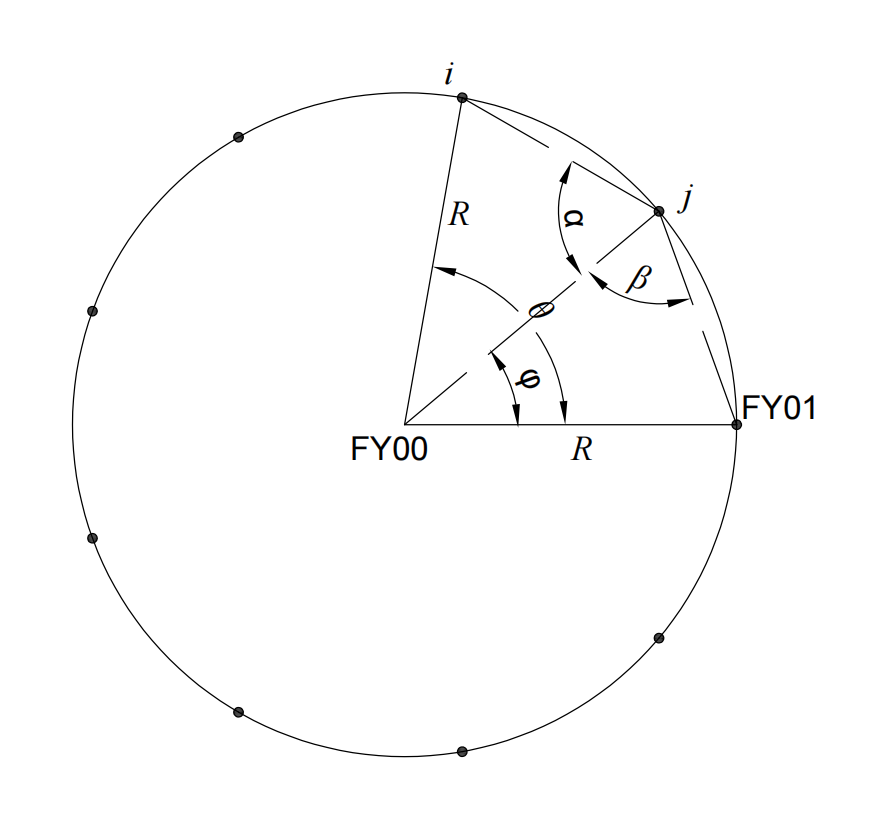
\includegraphics[width=0.9\textwidth]{../../figure/q1_1.png} 
        \caption{主动机与被动机排布的情况1}
        \label{q1_1}
    \end{minipage}
    \begin{minipage}{0.49\textwidth}
        \centering
        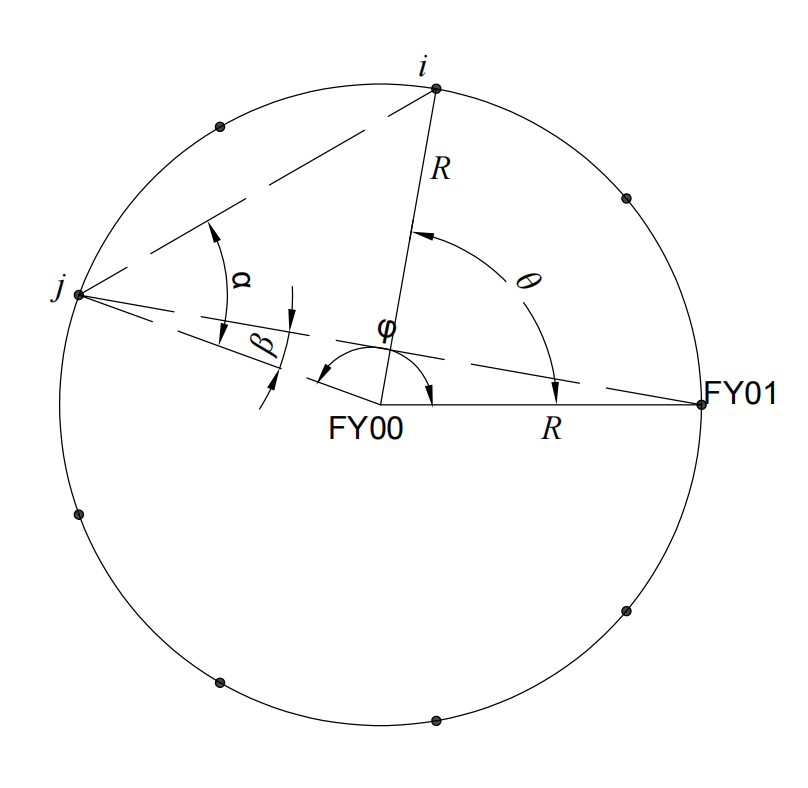
\includegraphics[width=0.86\textwidth]{../../figure/q1_2.png} 
        \caption{主动机与被动机排布的情况2}
        \label{q1_2}   
    \end{minipage}
    \caption*{\small 注:主动机发射的方向信息$\alpha$为$(i,0)$的夹角,$\beta$为$(0,1)$的夹角,图\ref{q1_2}同理。}
\end{figure}



\subsubsection{被动机定位模型求解}

将式(\ref{式1})相除可得

\begin{equation}
    \frac{\sin\beta}{\sin\alpha} = \frac{\sin(\pi - \varphi -\beta)}{\sin(\pi - \alpha - \theta + \varphi)}
\end{equation}

将上式整理得

\begin{equation}
    \tan\varphi= \frac{\cos\alpha + \cos(\alpha_2 +\theta)}{\sin(\alpha+\theta)- \sin\beta}
\end{equation}








\begin{figure}[htbp]
    \centering
    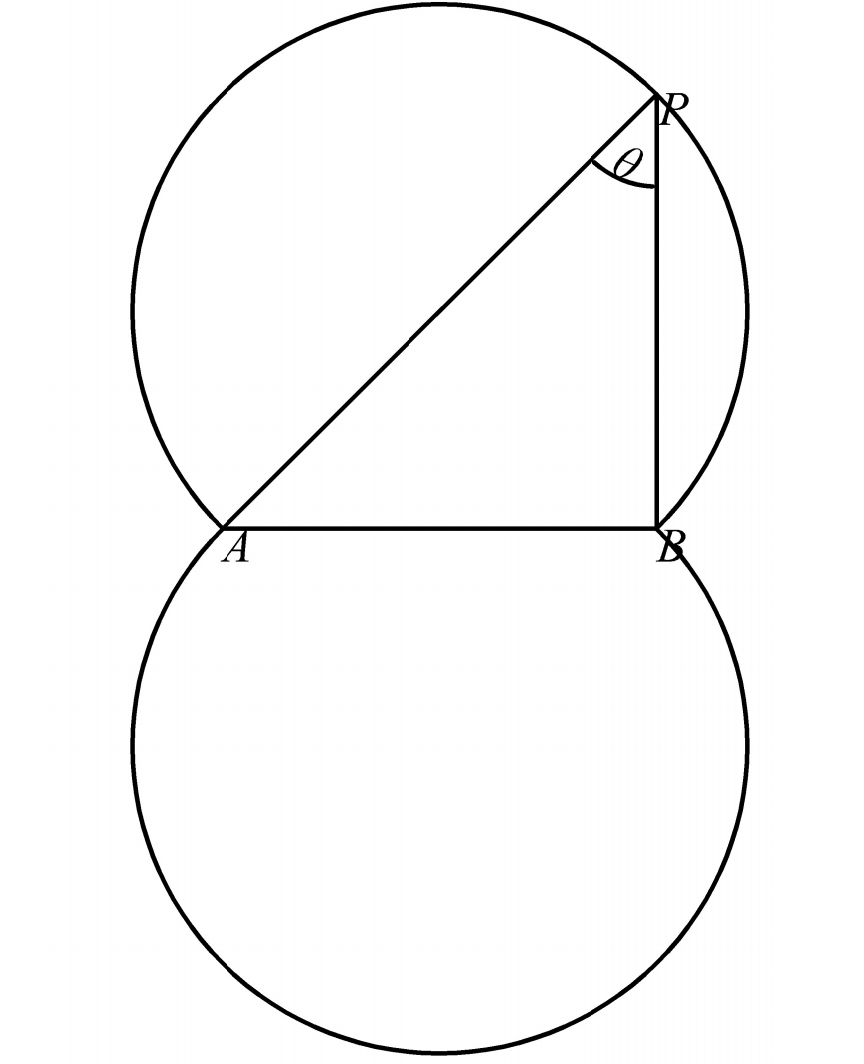
\includegraphics[width=0.5\textwidth]{../../figure/q1_3.png} 
    \caption{哈哈}  
    \label{q1_4}    
\end{figure}


\subsubsection{求解结果}




\subsection{问题二的模型建立与求解}
\subsubsection{模型建立}

我们先证明结论1:如果已知三个点及三点对于未知点的夹角,可以求出未知点的具体位置,证明过程如下:
假设我们已知点A、B的坐标,在平面上存在一点P,使得∠APB=theta,根据圆的性质:同一条弦 所对应的圆周角相等,可得P的轨迹是以AB为弦长的圆弧,可以确定P的轨迹为两条圆弧,此时点P的轨迹如图几所示,有无数个位置,只能确定其轨迹,无法确定具体位置,此时我们引入一点U,U的坐标已知,使得∠APU=theta,同理可得P的轨迹也是以AU为弦长的的两端圆弧,此时四段圆弧的轨迹如图几所示,可以看出此时四段圆弧有两个除A外的交点,此时便可以确定P的具体位置,再根据要求进一步确定P的位置。


\begin{figure}[htbp]
    \centering
    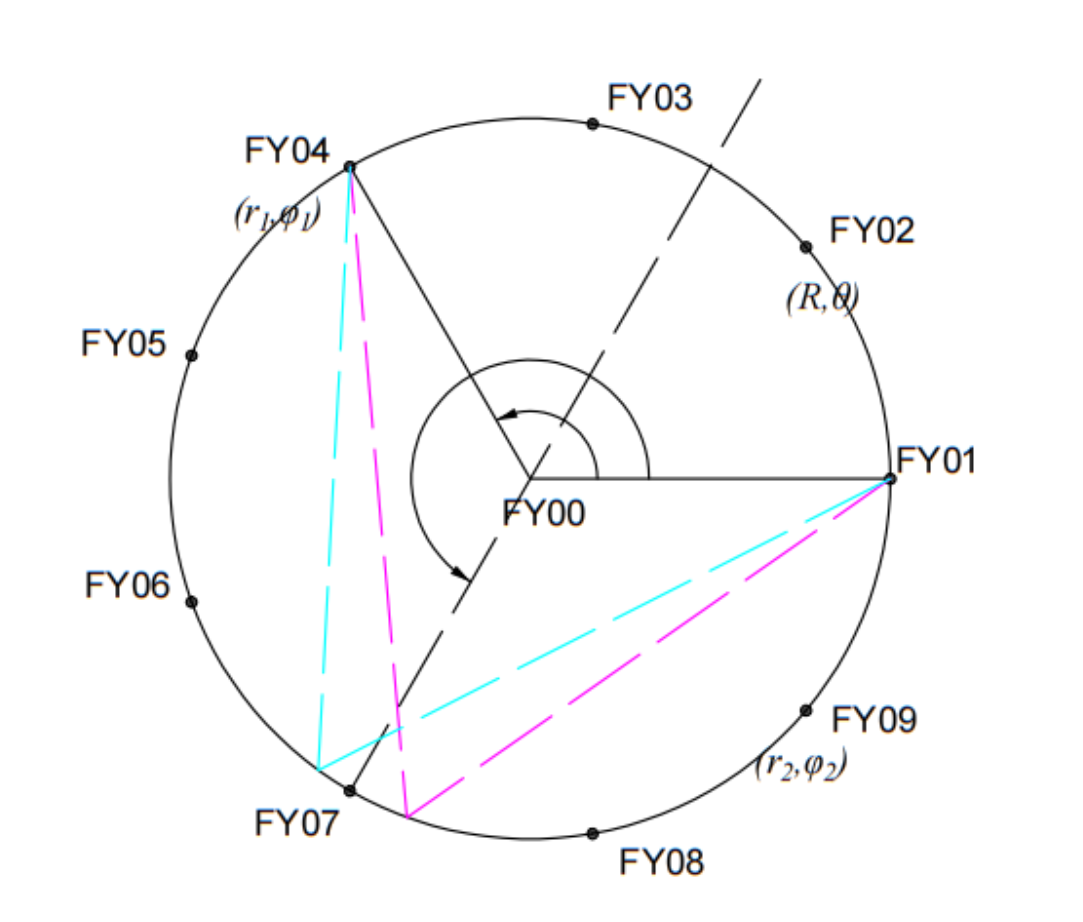
\includegraphics[width=0.5\textwidth]{../../figure/q1_4.png} 
    \caption{哈哈}
    \label{q1_3}   
\end{figure}

\subsubsection{问题求解}

再回到原题证明只需在已知FY00和FY01的作为主动机的基础上只需要一个无人机发射信号即可实现对无人机的有效定位,证明过程如下:
我们还是在问题一的原有极坐标系下已知FY00和FY01的坐标,假如我们要求i号机的具体位置,利用00和01对i号机的发射信号来确定:∠0i1,根据结论1我们可以知道i的轨迹为以01为弦长的两段圆弧,下面我们引入一架无人机j为主动机,我们可以得到发射信号∠1ij,我们可以得到i的轨迹为以1j为弦长的两端圆弧,我们便得到了两个关于i的运动轨迹,我们要同时满足i的两个不同的运动轨迹可知满足的点只有一个,但根据无人机编排在正九边形的端点上,我们很容易可以排除无效点的位置,从而得到真实的被动机的位置,实现对无人机的有效定位。



\subsubsection{求解结果}

\subsection{问题三的模型建立与求解}
\subsubsection{模型建立}
\subsubsection{问题求解}
\subsubsection{求解结果}


\subsection{问题四的模型建立与求解}
\subsubsection{模型建立}
\subsubsection{问题求解}
\subsubsection{求解结果}

% 模型的分析与检验
\section{模型的分析与检验}
\subsection{误差分析}
\subsection{灵敏度分析}


% 模型评价
\section{模型的评价}
\subsection{模型优点}
\begin{enumerate}
    \item ..
    \item ..
    \item ..
\end{enumerate}

\subsection{模型缺点}
\begin{enumerate}
    \item ..
    \item ..
\end{enumerate}

\subsection{改进方向}
\begin{enumerate}
    \item ..
    \item ..
\end{enumerate}

% 摘要
\bibliography{ref}

% 附录

\begin{appendices}

\section{运行结果}


\section{文件列表}
\begin{table}[H]
    \caption{程序文件列表}
    \centering
    \begin{tabularx}{\textwidth}{l X}
        \bottomrule
        文件名 & 功能描述 \\
        \midrule
        Enums.py & 自定义枚举类型 \\
        SaleFlow.py & 处理文档,将附件2的流水整理为便用的形式 \\
        SaleUtils.py & 处理表格、绘图等工具 \\
        code1.py & 问题一程序代码 \\
        code2.py & 问题二程序代码 \\
        code3.py & 问题三程序代码 \\
        \bottomrule
    \end{tabularx}
    \label{tab:文件列表}
\end{table}

\section{代码}
问题1代码
\lstinputlisting[language=python]{../../code/code1.py}
问题2代码
\lstinputlisting[language=python]{../../code/code2.py}
问题3代码
\lstinputlisting[language=python]{../../code/code3.py}

\end{appendices}

\end{document}